\chapter{Umweltbelastung}
Durch das erreichte Stadium der technischen Entwicklung in Industrie, Gewerbe und Landwirtschaft verändert und belastet der Mensch die Umwelt.
Die Umweltbelastung kann viele Ursachen haben, möglicherweise sind bessere Lösungen nicht umsetzbar oder wirtschaftlich nicht attraktiv.
Die Umweltbelastung entsteht auf verschieden Ebenen, die sich in ihrer Gegebenheit unterscheiden.
Es gibt energetischen Belastungen, wie Strahlen, Lärm und Erschütterungen.
Es gibt Umweltbelastungen durch feste Stoffe wie Abfälle die durch Bau und Abbruch entstehen, Abfälle aus Produktionen und Abfälle aus der Gewinnung von Bodenschätzen.
Auch flüssige Stoffe belasten die Umwelt. Sie entstehen durch Chemie Fabriken, Reste von Medikamenten die durch den Urin in das Abwasser gelangen oder durch Umweltkatastrophen bei der Sich das Wasser mit andren Stoffen vermischt.
Ein Beispiel hierfür könnte ein Erbebben sein, welches ein Atomkraftwerk beschädigt und radioaktives Wasser ausläuft.
Die größte Umweltbelastung ist aber die gasförmige Verschmutzung, welche die Luft verschmutzt.
Durch unsachgemäßes Recycling kann eine Luftverschmutzung entstehen.
Wenn zum Beispiel feste Stoffe verbrannt werden um nicht brennbare Stoffe wieder zu verwerten.
Das ist der Fall bei Stromkabeln wenn die Isolierung verbrannt wird um das wertvolle Kupfer zu gewinnen.
Die Luftverschmutzung ist die eine große Ursache für Krankheiten und den vorzeitigen Tod von Menschen.
Sie kann in den Körper eindringen und schwerwiegende Krankheiten auslösen.
Luftverschmutzung entsteht bei Tierhaltung sowie durch den Einsatz von Pestiziden. 

Die Hauptursache sind aber Abgase die bei der Verbrennung von fossilen Kraftstoffen entstehen. 
Ein großer Träger bei der Verbrennung von fossilen Kraftstoffen sind Kraftfahrzeuge.

\chapter{Kraftfahrzeuge}
\textit{Als Kraftfahrzeuge im Sinne dieses Gesetzes gelten Landfahrzeuge, die durch Maschinenkraft bewegt werden, ohne an Bahngleise gebunden zu sein.}
\footnote{Straßenverkehrsgesetz, § 1 Abs. 2}

Da Kraftfahrzeuge Landfahrzeuge sind gehören Flugzeuge, Schiffe oder Boote nicht zu der Kategorie, obwohl sie durch Maschinenkraft bewegt werden.
Auch Züge oder Trambahnen gehören nicht in in die Kategorien, da sie an Bahngleise gebunden sind.

Moderne Kraftfahrzeuge werden aus folgenden Teilsysteme gebildet:
\begin{itemize}
	\item Antriebseinheit
	\item Energieübertragungseinheit
	\item Stütz- und Trageeinheit
	\item Steuerungs- und Regelungseinheit
	\item Arbeitseinheit
\end{itemize}


\begin{figure}[h!]
	\caption{Teilsysteme des Kraftfahrzeugs}
	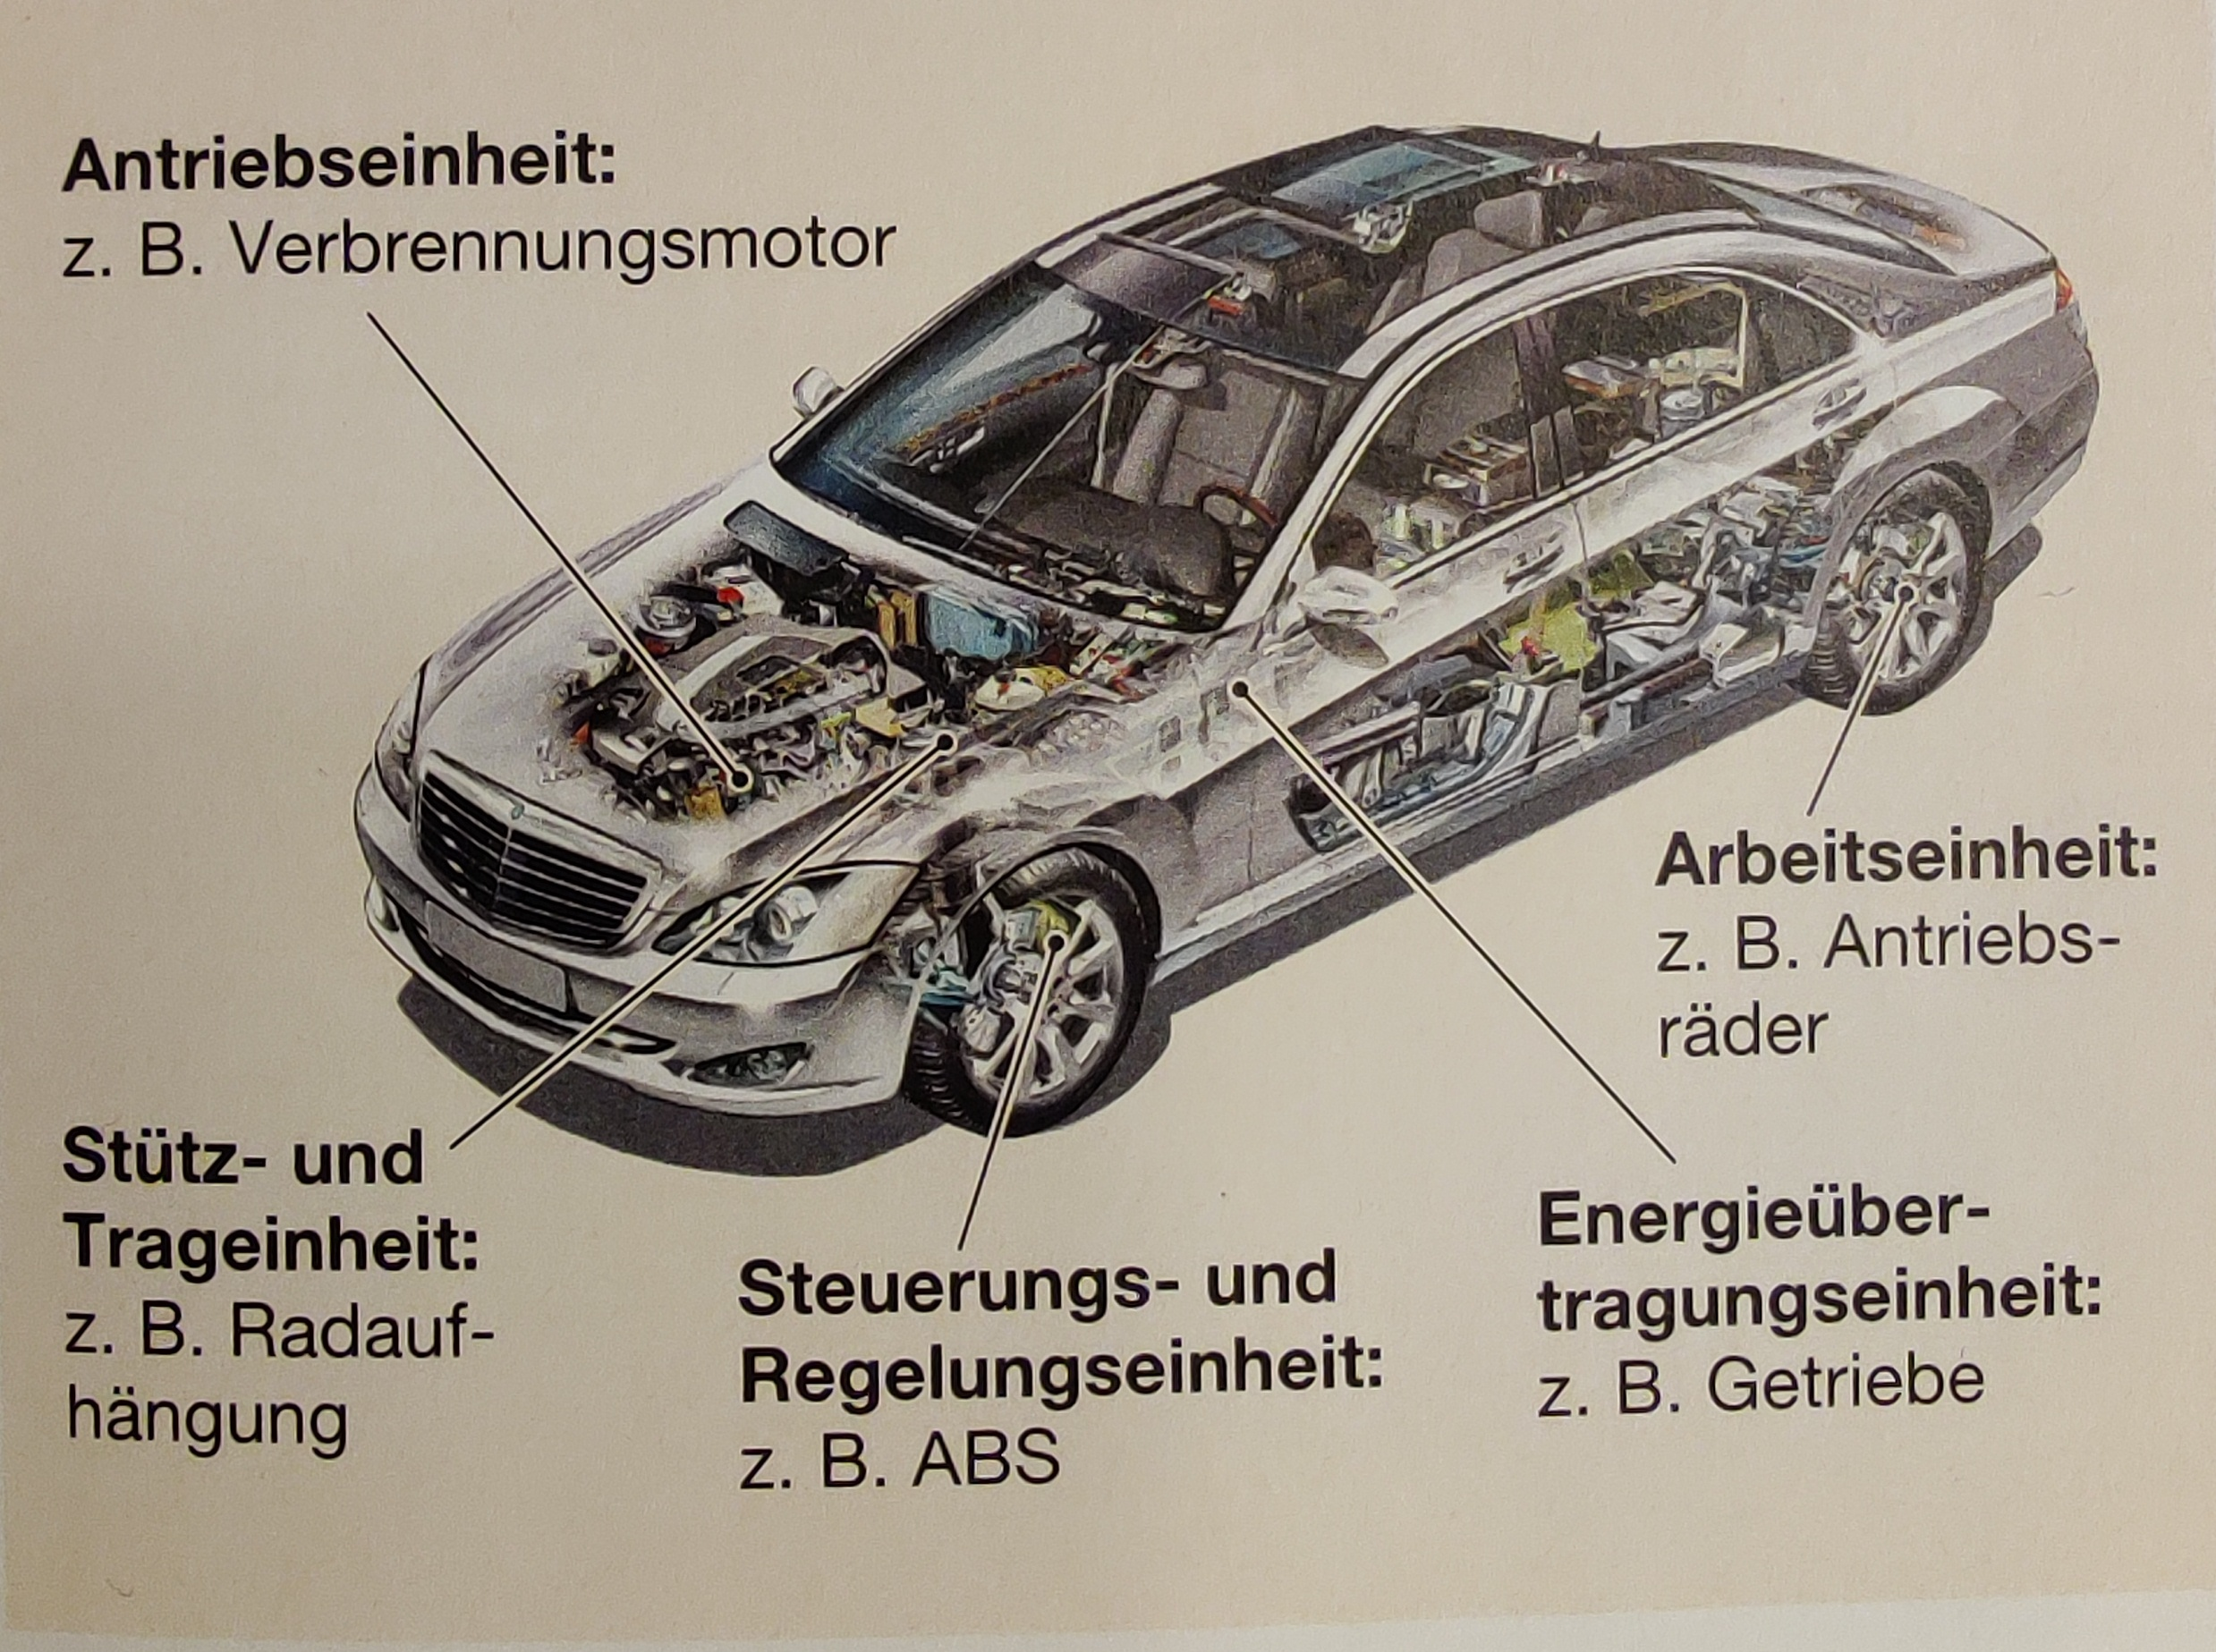
\includegraphics[scale=0.1]{assets/figures/Teilsysteme des Kraftfahrzeugs.jpg}
	\begin{flushleft}
		Quelle: Westermann S. 19
	\end{flushleft}
	\label{fig:birds}
\end{figure}


\subsection{Antriebseinheit}
Die Antriebseinheit wandelt die zugeführte Energie in die erforderliche Antriebsenergie um.
\footnote{Westermann S. 19}
Diese Umwandlung wird im Motor durchgeführt.
Hauptsächlich werden Elektro- und Verbrennungsmotoren eingesetzt.

Verbrennungsmotoren unterscheiden sich von Elektromotoren durch ihre Energieerzeugung.
Die Energieerzeugung wird durch die Verbrennung von Kraftstoff erzeugt.
Dazu wird ein Kraftstoff Luftgemisch in einem Brennraum mit Kolben zur Verbrennung verwendet.
Durch die Verbrennung steigt der Druck im Brennraum stark an und bewegt einen Kolben.

\subsection{Arbeitseinheit}
Die Arbeitseinheit ist die Verbindung zwischen den Antriebsrädern und der Fahrbahn.
Durch die Bewegung der Antriebsrädern wird das Kraftfahrzeug in Bewegung gesetzt.

\subsection{Energieübertragungseinheit}
Die Energieübertragungseinheit leitet die Energie in der geforderten Bewegungsart und Bewegungsgeschwindigkeit zur Arbeitseinheit weiter.
\footnote{Westermann S. 19}

Energieübertragungseinheiten sind Baugruppen einer Maschine, die zur Übertragung von Energie in benötigt werden. 
Beispiel hierfür sind Kabel zur die Elektrische Engergie leiten, aber auch Wellen, Zahnräder oder Riemen welche mechanische Energie weiterleiten.

\subsection{Stütz- und Trageeinheit}
Am Kraftfahrzeug ist die Stütz- und Trageeinheit der Rahmen oder oder der selbsttragende Aufbau.
Diese haben hauptsächlich die Aufgabe, die Teilsysteme aufzunehmen und zu einer Einheit zu verbinden.
\footnote{Westermann S. 19}


\subsection{Steuerungs- und Regelungseinheit}
Die Steuerungs- und Regelungseinheit Beeinflusst die Stoff- und Energieumsetzung durch Informationsverarbeitung
\footnote{Westermann S. 19}

\subsubsection{Steuerungseinheit}
Bei der Steuerungseinheit werden verschiedene Eingangsgrößen durch das System ein oder mehrere Ausgangsgrößen erzeugt.
Beispiele für Steuerungen sind:
\begin{itemize}
	\item Klimaanlage: Es wird eine Solltemperatur eingestellt.
	      Die Klimaanlage kühlt konstant. 
	      Die Klimaanlage kühlt solange mit dieser eingestellten Temperatur bis sie verändert wird.
	      Die Umgebungstemperatur wird nicht berücksichtigt.
	\item Licht: Der Schalter wird betätigt und das Licht wird eingeschaltet.
	      Das Licht bleibt permanent eingeschaltet.
	      Das Licht geht erst aus wenn der Schalter ausgeschaltet wird.
	      Das Umgebungslicht wird nit berücksichtigt.
\end{itemize}
\subsubsection{Regelungseinheit}
Bei einer Regelungseinheit werden die Eingangsgrößen mit einem Sollwert verglichen und so lange angepasst bis der Sollwert erreicht wird.
Beispiele für Regelungen sind:
\begin{itemize}
	\item Klimaautomatik: es wird eine Solltemperatur eingestellt.
	      Es wird gemessen wie warm oder wie Kalt die Temperatur ist.
	      Sollte die Temperatur unter der Solltemperatur liegen, wird die Klimaautomatik auf Heizen gestellt.
	      Sollte die Temperatur über der Solltemperatur liegen, wird die Klimaautomatik auf Kühlen gestellt.
	\item Lichtautomatik: Es gibt eine Schwelle bei der das Licht eingeschaltet werden soll.
	      Es gemessen wie hell das Umgebungslicht ist. 
	      Sollte das Umgebungslicht zu gering sein wie \ac*{zb} im Tunnel oder bei Dämmerung wird das Licht eingeschaltet. 
	      Sobald das Umgebungslicht wieder hell genug ist \ac*{zb} beim verlassen des Tunnels oder bei Sonnenaufgang, wird das Licht wieder ausgeschaltet.
\end{itemize}


\section{Fahrzeugklassen}

Kraftfahrzeuge können Bauartbedingt in Kategorien eingeordnet werden.
Die EU Kommission hat hat hierfür acht Klassen definiert.\footnote{VERORDNUNG (EU) Nr. 678/2011 DER KOMMISSION
	vom 14. Juli 2011, TEIL A ABS.1 - https://eur-lex.europa.eu/eli/reg/2011/678/oj?locale=de}

\begin{itemize}
	\item Klasse L: Leichte ein- und zweispurige Kraftfahrzeuge
	\item Klasse M: Vorwiegend für die Beförderung von Fahrgästen und deren Gepäck ausgelegte und gebaute Kraftfahrzeuge
	\item Klasse N: Vorwiegend für die Beförderung von Gütern ausgelegte und gebaute Kraftfahrzeuge
	\item Klasse O: Anhänger, die sowohl für die Beförderung von Gütern und Fahrgästen als auch für die Unterbringung von Personen ausgelegt und gebaut sind
	\item Klasse S: unvollständige Fahrzeuge, die der Unterklasse der Fahrzeuge mit besonderer Zweckbestimmung zugeordnet werden soll
	\item Klasse R: Anhänger, die in der Land- und Forstwirtschaft verwendet werden
	\item Klasse S: Maschinen, die in der Land- und Forstwirtschaft zum Einsatz kommen und gezogen werden
	\item Klasse T: Zugmaschinen, die in der Land- und Forstwirtschaft verwendet werden wie Traktoren
	\item Klasse C: Zugmaschinen, die in der Land- und Forstwirtschaft verwendet werden und auf Ketten laufen wie ein Bagger
\end{itemize}

Die relevantesten Klassen sind M und N.

\subsection{Klasse M}
In der Klasse M werden Kraftfahrerzegge eingeordnet die für die Beförderung von Personen und Gepäck zuständig sind und mindestens 4 Räder haben sowie eine Hochgeschwindigkeit von über 25 \ac{kmh} haben.
\newline
Die Klasse M wird spaltet sich in 3 Unterklassen auf.
\begin{itemize}
	\item {Klasse M1}
	\item {Klasse M2}
	\item {Klasse M3}
\end{itemize}
\subsubsection{Klasse M1}
Kraftfahrzeuge der Klasse M1 haben über die Eigenschaften der Klasse M noch folgende weitere Eigenschaften:
\begin{itemize}
	\item {nicht mehr als 8 Sitzplätze und 1 Platz für den Fahrer}
	\item {keine Stehplätze}
	\item {zulässiges Gesamtgewicht von maximal 3,5 \ac{t}}
\end{itemize}

In der Klasse M1 Kraftfahrzeuge wie Personenkraftwagen(Limousine, Cabrio) und Wohnmobile zu finden.

\subsubsection{Klasse M2}
Kraftfahrzeuge der Klasse M2 haben über die Eigenschaften der Klasse M noch folgende weitere Eigenschaften:
\begin{itemize}
	\item {mehr als 8 Sitzplätze}
	\item {zulässiges Gesamtgewicht von maximal 5 \ac{t}}
\end{itemize}

In der Klasse M2 sind Kraftfahrzeuge wie ein Eindecker-Bus bis 5 \ac{t} oder ein Doppeldecker-Bus bis 5 \ac{t} zu finden.

\subsubsection{Klasse M3}

Die dritte Unterklasse der Klasse M ist M3.

Kraftfahrzeuge der Klasse M3 haben über die Eigenschaften der Klasse M noch folgende weitere Eigenschaften:
\begin{itemize}
	\item {mehr als 8 Sitzplätze}
	\item {zulässiges Gesamtgewicht von über 5 \ac{t}}
\end{itemize}

In der Klasse M3 sind Kraftfahrzeuge wie ein Eindecker-Bus über 5 \ac{t} oder Doppeldecker-Bus über 5 \ac{t} zu finden.

\subsection{Klasse N}
In der Klasse N werden Kraftfahrerzegge eingeordnet die für die Beförderung von Gütern zuständig sind und mindestens 3 Räder haben sowie ein zulässiges Gesamtgewicht von über 1 \ac{t} haben.
Die Klasse N spaltet sich in 3 Unterklassen auf.
\begin{itemize}
	\item {Klasse N1}
	\item {Klasse N2}
	\item {Klasse N3}
\end{itemize}

\subsubsection{Klasse N1}
Fahrzeuge zur Güterbeförderung mit einer zulässigen Gesamtmasse bis zu 3,5 \ac{t}.
In der Klasse N1 sind Kraftfahrzeuge die in dicht besiedelten Regionen gut zurecht kommen, wie Paketzusteller oder Fahrzeuge der Post.


\subsubsection{Klasse N2}
Fahrzeuge zur Güterbeförderung mit einer zulässigen Gesamtmasse von zu 3,5 \ac{t} bis 12 \ac*{t}.
In der Klasse N2 sind Kraftfahrzeuge die regional Güterbefördern, dies könnten Kraftfahrzeuge die Waren aus einem Zentrallager in die Filialen transportieren. 
Diese Kraftfahrzeuge sind darauf ausgelegt hunderte Kilometer zurückzulegen.


\subsubsection{KLasse N3}
Fahrzeuge zur Güterbeförderung mit einer zulässigen Gesamtmasse von mehr als 12 \ac{t}.
In der Klasse N3 sind Kraftfahrzeuge die überregional Güterbefördern, wie ein Kraftfahrzeug das große Mengen an Ladung fassen kann und darauf ausgelegt sind tausende Kilometer zurückzulegen.

\section{Umweltbelastungen von Kraftfahrzeugen}
Kraftfahrzeuge belasten die Umwelt auf verschiedene Arten. Hierunter fallen 
die Erzeugung von Rohstoffen für Materialien die für die Produktion von Kraftfahrzeugen benötigt werden, 
die tatsächliche Produktion von Kraftfahrzeugen,
der Betrieb von Kraftfahrzeugen,
sowie die Entsorgung von Kraftfahrzeugen.

Gerade aber der Betrieb von Kraftfahrzeugen belastet die Umwelt durch die verschieden Arten von Schadstoffen.
Unterschieden wird durch die Verbrennung von Kraftstoff freigesetzten Schadstoffe in Form von Verbrennungsabgasen aber auch durch Partikel die durch den Abrieb der Reifen oder Bremsbeläge freigesetzt werden.
Aber auch die Infrastruktur belastet die Umwelt.

\subsection{Verbrennungsabgase}
Die größten Anteile der giftigen Schadstoffe die durch die Verbrennung von Kraftstoff entstehen sind:
\begin{itemize}
	\item {\ac{CO}}
	\item {\ac{NO}}
	\item unverbrannte Kohlenwasserstoffe (HC)
	\item Feinstaub
\end{itemize}
Es gibt auch ungiftige Stoffe die durch die Verbrennung erzeugt werden wie z.B. Wasser, \ac{CO2}.
Die durch die Verbrennung entstehenden Abgase werden in einer Abgasanlage in die Umwelt geleitet.
In der Abgasanlage werden auch gifte Gase im Rahmen des technisch Möglichen aufspalten und umgewandelt um den negativen Einfluss zu verringern.

\subsection{Abrieb}

\subsection{Infrastruktur}



\section{Wie kann autonomes Fahren die negativen Auswirkungen reduzieren?}
% !!! hier kann man Beispiele aufführen, wie zb Bus, PKW, LKW; Traktor
% !!! Wie groß ist der Anteil der Kraftfahrzeuge in den Klassen in Deutschland?
% !!! Warum und wie blesatst jede Klasse die Umwelt?
% !!! PKW durch unnötige Kurzstecke
% !!! Sinnloses laufenlassen von LKW
% !!! Zustellungen von Gütern
% !!! Leerfahrten


\subsection{Autonomes Fahren}

!!! Was sind autonome fahrzeuge?
!!! Welche 


Beim autonomen Fahren, fährt ein \ac{Kfz} Verwaltungsgefäß selbständig.
Für \ac{Kfz} wurden von der \ac{SAE} Institut in der Norm SAE J3016\footnote{SAE J3016\textunderscore202104 - https://www.sae.org/standards/content/j3016\textunderscore202104} Automatisierungsgrade definiert.
\begin{itemize}
	\item Stufe 0 (Keine Automation)
	\item Stufe 1 (Assistenzsysteme)
	\item Stufe 2 (Teilautomatisierung)
	\item Stufe 3 (Bedingte Automatisierung)
	\item Stufe 4 (Hochautomatisierung)
	\item Stufe 5 (Vollautomatisierung)
\end{itemize}
\subsubsection{Was passiert in den Stufen?}
Die Stufen unterscheiden sich im wesentlichen nur durch die Anzahl der Automatisierungsgrade.

\vspace{0.5cm}

In der Stufe 0 (Keine Automation):
\begin{itemize}
	\item keine Assistenzsysteme
	\item \ac{Kfz} kann keine Fahraufgaben übernehmen
	\item Fahrer ist unter permanenter Kontrolle
\end{itemize}

\vspace{0.5cm}

In der Stufe 1 (Assistenzsysteme):
\begin{itemize}
	\item Assistenzsysteme wie \ac{GRA} oder eine Berganfahrhilfe
	\item Fahrer hat eine passive Unterstützung bei Fahraufgaben
	\item \ac{Kfz} kann keine Fahraufgaben übernehmen
	\item das \ac{Kfz} ist unter permanenter Kontrolle des Fahrers
\end{itemize}

\vspace{0.5cm}

In der Stufe 2 (Teilautomatisierung):
\begin{itemize}
	\item Assistenzsysteme, wie der Spurführungsassistent oder Stauassistent
	      \begin{itemize}
		      \item automatisch bremsen
		      \item automatisch beschleunigen
		      \item automatisch lenken
	      \end{itemize}
	\item \ac{Kfz} kann Fahraufgaben teilautomatisiert übernehmen
	\item Fahrer kann sich für kurze Zeit von den Fahraufgaben abwenden
	\item Fahrer muss jeder Zeit die Fahraufgabe übernehmen können
\end{itemize}

\vspace{0.5cm}

In der Stufe 3 (Bedingte Automatisierung):
\begin{itemize}
	\item hochautomatisierte Assistenzsysteme
	\item \ac{Kfz} kann Fahraufgaben unter bestimmten Voraussetzungen vollständig übernehmen
	\item Fahrer kann sich unter bestimmten Voraussetzungen dauerhaft von den Fahraufgaben abwenden
	\item Fahrer muss innerhalb wenigen Sekunden die Fahraufgabe übernehmen können
\end{itemize}

\vspace{0.5cm}

In der Stufe 4 (Hochautomatisierung):
\begin{itemize}
	\item hochautomatisierte Assistenzsysteme
	\item \ac{Kfz} kann Fahraufgaben in hochkomplexen Verkehrssituationen vollständig übernehmen
	\item Fahrer dauerhaft von den Fahraufgaben abwenden
	\item Fahrer muss fahrtüchtig sein, um im Bedarfsfall die Fahraufgabe übernehmen zu können
\end{itemize}

\vspace{0.5cm}

In der Stufe 5 (Vollautomatisierung):
\begin{itemize}
	\item hochautomatisierte Assistenzsysteme
	\item \ac{Kfz} übernimmt alle Fahraufgaben vollständig
	\item Fahrer ist nicht erforderlich
	\item alle Personen im Wagen werden zu Passagieren
\end{itemize}

\subsection{Umwelteinflüsse}

\textit{Umwelt bezeichnet etwas, mit dem ein Lebewesen in Beziehungen steht.}\footnote{Ludwig Trepl: Allgemeine Ökologie. Band 1: Organismus und Umwelt. Frankfurt/M., Lang: 106ff.; vgl. 1. Uexküll, Jakob von 1909: Umwelt und Innenwelt der Tiere. Springer, Berlin 2005.}

Einfluss ist eine Wirkung auf ein Subjekt, das eine bestimmte Umweltbedingung erfüllt.

Umwelteinflüsse sind daher eine Wirkung auf Lebewesen.

\vspace{.5cm}
Unter Umwelteinflüssen von \ac{Kfz} fallen \ac{ua}:
\begin{itemize}
	\item benötigte Flächen, für Infrastruktur, Parkplätze \ac{usw}
	\item der Verbrauch von Stoffen um Energie für \ac{Kfz} zu erzeugen oder Betriebszustände für Fahrbahnen herzustellen
	\item der Ausstoß von Gasen die \ac{zb} durch Verbrennung von Kraftstoff oder beim Laden einer Batterie entstehen
	\item der Verlust von Betriebsmitteln durch Leckage an Systemen
	\item der Ausstoß von festen Stoffe wie \ac{ua} Bremsstaub oder Abrieb der Reifen der beim Bremsen entsteht
	\item Wärme und Schall durch die Umwallung von Energie oder Reibung von Komponenten die beim Betrieb des \ac{Kfz} entstehen
	\item Licht zur Beleuchtung der Fahrbahn oder Absicherung der Verkehrsführung
\end{itemize}


\subsection{Feinstaub}
!!! Warum entsteht Feinstaub?
!!! Wann und wie entsteht Feinstaub?


Feinstaub entsteht durch natürlichen Ursprung oder wird durch menschliches Handeln erzeugt.


Der primäre Feinstaub entsteht direkt aus der Quelle wie durch eine Verbrennung.  

Der sekundäre Feinstaub entsteht durch eine chemische Reaktionen in der Atmosphäre aus gasförmigen Substanzen, 
wie Schwefel- und Stickstoffoxiden, Ammoniak oder Kohlenwasserstoffen.

Wichtige durch menschliches Handeln verursachte Feinstaubquellen sind: 
\begin{itemize}
	\item \ac{Kfz}
	\item Kraft- und Fernheizwerke
	\item Abfallverbrennungsanlagen
	\item Heizungen in Wohnhäusern
	\item bestimmte Industrieprozesse
\end{itemize}

In urbanen Regionen sind vor allem der Straßenverkehr und Bautätigkeiten große Feinstaubquellen.

Hierbei entsteht Feinstaub nicht nur aus dem Verbrennungsprozess in die Luft, sondern auch durch Bremsen-, Reifen- und Fahrbahnabrieb. 
Auch die Aufwirbelungen des Staubes von der Straßenoberfläche tragen dazu bei. 
Wichtige natürliche Quellen für Feinstaub sind Emissionen aus Vulkanen und Meeren aber durch Bodenerosionen, Wald- und Buschfeuer oder 
bestimmte biogene Gemische von Viren, Sporen, Bakterien oder Pilzen.

